\subsubsection{Recolecion de la informacion de los lugares}
% \label{subs:Los lugares}

En primer lugar se recolectó la información de los lugares que la aplicación contendrá  de forma inicial, al igual que para recolectar las rutas se hizo uso de un \emph{GPS Garmin Nuvi 1300}, el cual cuenta con la opción de guardar locaciones como favoritos, entonces solo fue necesario estar cerca del lugar que se desea guardar y activar esa opción del GPS, este guarda la información en un archivo \emph{.gpx} y con la ayuda de \emph{QGIS} se genero el archivo shapefile correspondiente.\\

Posteriormente es necesario pasar la información geoespacial del shapefile a la base de datos, para esta tarea se hizo uso de una herramienta disponible para postgres, \emph{shp2pgsql}, que permite la conversión de un archivo shapefile a un archivo sql.

% $ shp2pgsql -s 4326 -I -S -c -d ~/Documents/places.shp > places.sql
\begin{verbatim}
  $ shp2pgsql -s 3785 -I -S -c -d ~/Documents/places.shp > places.sql
\end{verbatim}

Con el anterior comando se tiene como resultado un archivo \emph{.sql}, el cual es ingresado en la base de datos ya configurada, de esta forma nuestra base de datos para a contener una tabla geoespacial con datos de tipo \emph{POINT}, los cuales representan los lugares dentro del campus de la UMSS.\\

% \begin{verbatim}
%   $ shp2pgsql -s 4326 -I -S -c -d ~/Documents/ways.shp > ways.sql
% \end{verbatim}
%
% De la misma forma es necesario pasar la información de las rutas contenidas en un archivo shapefile a un archivo sql, en este caso creará una tabla \emph{WAYS}.\\

El archivo \emph{sql} resultante es usado para popular la base de datos con la información inicial de los lugares que contiene el campus universitario, para tal tarea se usó el siguiente comando.\\
% Los archivos resultantes \emph{sql} son usados para popular la base de datos .\\

\begin{verbatim}
  $ psql -d db_ubikate -U db_admin -f /Documents/places.sql
\end{verbatim}

\begin{figure}[H]
  \begin{center}
    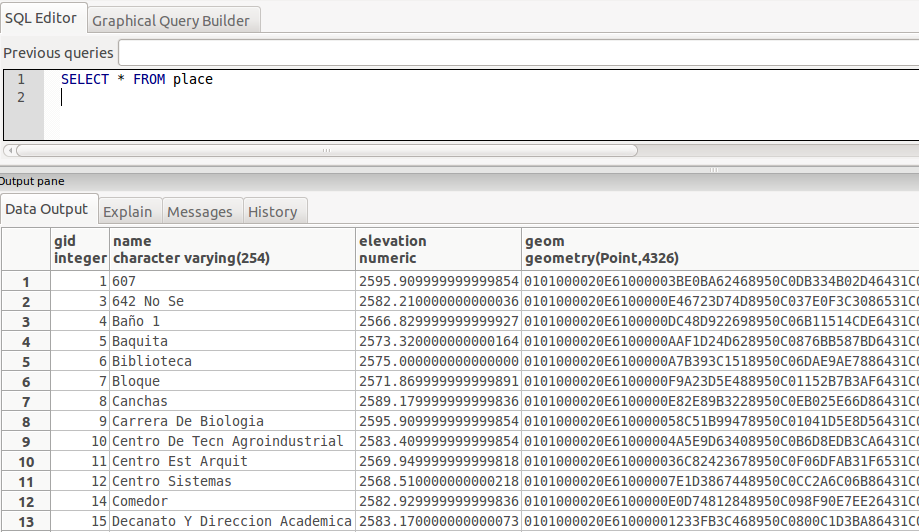
\includegraphics[width=1\textwidth]{iteration1/postgres_places}
    \caption{Herramienta gráfica de PostgreSQL (\emph{pgAdmin}).}
    \label{fig:postgres_places}
    \caption*{Fuente: Elaboración propia}
  \end{center}
\end{figure}
 % con la tabla de Lugares desplegada.

En la figura \ref{fig:postgres_places} se puede observar que la columna \emph{Elevation} contiene datos que el GPS Garmin Nuvi 1300 genera al momento de guardar un punto, en el presente caso es irrelevante.\\


Una vez que se tiene populada la base de datos con la informacion de los lugares es necesario implementar el como se comunicara el backend con el frontend, este como ya se explico se implementara un Servicio Web basado en un API REST.\\



\subsubsection{Implementación del REST API}
\label{subs:Implementacion del REST API}



El servidor necesita reconocer las peticiones que le llegan del cliente, para lo cual es necesario ``mapear'' un URI a una acción específica, las cuales ya están preparadas para comunicarse con la base de datos, no hay restricción en la declaración de las URIs pero para una mejor comprensión del API que se está desarrollando es necesario seguir convenciones que aseguran que cualquier desarrollador pueda comprender el API presentado y pueda ser fácilmente consumido por cualquier aplicación que requiera acceder a la información que disponible, un API REST es el que cumple con estas características.
En primer lugar es necesario crear las URIs que serán ``entendidas'' por el servidor, esto se logra declarando en el servicio creado con \emph{Express.JS}, tal como se puede apreciar en el siguiente bloque de código, cada URI se lo relaciona a un modelo en específico de acuerdo a la acción que se requiere, tal como se puede observar en el cuadro \ref{tab:rest} las URIs declaradas en el API cumplen con tal característica.\\


% \begin{minted}{js}[label=express_api,caption=Declarando API REST con ExpressJS]
\begin{center}
  \begin{lstlisting}[label=express_api,caption=Declarando API REST con ExpressJS]

        const router = express.Router();
        router.get('/', places.getAll);
        router.get('/:id', places.getPlace);
        router.post('/', places.newPlace);
        router.put('/:id', places.editPlace);
        router.delete('/:id', places.deletePlace);

        app.use('/api/v1/places', router);

  \end{lstlisting}
\end{center}
% \end{minted}

% En el código

  %
  % Para lograr todo este comportamiento  es necesario declarar, en el archivo
  % que controla las rutas dentro de la aplicación, \textbf{routes}, que el
  % recurso \textbf{user} es \emph{restful}, tal como se muestra en la figura \ref{fig:rest}\\

  % \begin{figure}[!hbp]
  %   \begin{center}
  %     \caption[REST - routes.rb]{config/routes.rb}
  %     \label{fig:rest}
  %     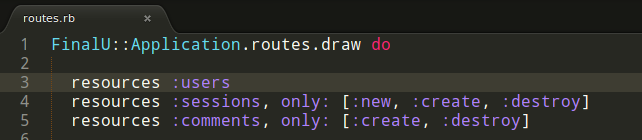
\includegraphics[width=1\textwidth]{rest}
  %     \caption*{Fuente: }
  %   \end{center}
  % \end{figure}

  El cuadro \ref{tab:rest} muestra como se puede leer las peticiones al API de \textbf{places}, las acciones mostradas son las que se pueden encontrar en un API REST pero no es necesario declararlas todas para considerar a que un API es restful.\\


  \begin{table}[H]
    \begin{center}

      \begin{tabularx}{0.75\textwidth}{ l l l  X }
        \toprule
        \multicolumn{1}{c}{\textbf{HTTP}} &
        \multicolumn{1}{c}{\textbf{URI}}  &
        % \multicolumn{1}{c}{\textbf{C}}  &
        \multicolumn{1}{c}{\textbf{ACCI\'ON}} &
        \multicolumn{1}{c}{\textbf{USADO PARA}}  \\
        \multicolumn{1}{c}{\textbf{request}} & & & \\

        \midrule
        GET     &  /places    &  index    & devuelve una lista con todos los lugares\\
        POST    &  /places    &  create   & inserta un nuevo lugar en la bd\\
        GET     &  /places/1  &  show     & muestra el lugar con identificador \emph{1}\\
        PUT     &  /places/1  &  update   & actualiza los datos de un lugar específico\\
        DELETE  &  /places/1  &  delete   & elimina el lugar con id = 1 de la bd\\
        \bottomrule
      \end{tabularx}

      \caption[recursos REST]{REST URIs para los lugares}
      \label{tab:rest}

      \caption*{Fuente: Elaboración propia}
    \end{center}
  \end{table}

  % Tal como se ve en el cuadro \ref{tab:rest}, Rails maneja los request HTTP de acuerdo con
  % el tipo de llamada que se realice, este trabajo lo realiza el \textbf{router},
  % que reconoce las URLs y los despacha a una \textbf{acción} del controlador,
  % todo este proceso ya está implementado en el núcleo de Rails por lo tanto  es automático y el programador
  % no necesita más configuración que la mostrada en la figura \ref{fig:rest},
  % obedeciendo al principio de \emph{Convención sobre configuración}\\

  % % no son más que métodos dentro del \emph{user\_controller.rb}
  % el cual
  % es parte del controlador de la arquitectura MVC.\\

  % The Rails router recognizes URLs and dispatches them to a controller’s action. It can also generate paths and URLs, avoiding the need to hardcode strings in your views.

  Por ejemplo, si se genera una petición GET hacia la direccion
  \mbox{\emph{/places/1}}  el servidor interpreta la dirección y responde
  mostrando la información del lugar “1” y en cambio si se genera
  una petición \emph{PUT} a la misma direccion \emph{/places/1} se ejecuta la acción \textbf{update} y se actualizan los datos del lugar ``1''. \\

  % \textbf{usuarios} actualizando la información del usuario “1”. \\

  Siguiendo la convención de un API REST ayuda a entender el flujo que tiene un recurso,
  las URL son legibles y únicos para cada recurso. Por lo tanto la implementación   de los recursos se hace de forma más limpia y ordenada, situaciones que son   claves para el mantenimiento y la extensibilidad del sistema. \\


Una vez implementado el servicio web, necesitamos empezar con el desarrollo del frontend de la aplicacion, que como ya se explico se usara \emph{EmberJS} para esta tarea. \\


\subsubsection{Mostrar los lugares}


\emph{EmberJS} tiene que consumir la informacion del API implementado, por lo tanto se hara una llamada \emph{GET} al URI \emph{places/}, dentro de la estructura de \emph{EmberJS} se tiene que implementar en el \emph{Router} dedicado al URI correspondiente. El siguiente metodo es el encarado de hacer la llamada y obtener la lista de lugares del API

\begin{center}
  \begin{lstlisting}[label=model_places_index,caption=Obtener la lista de lugares del API]

    model() {
        var url = (ENV.APP.API_HOST || '') + '/api/v1/places/';
        return jQuery.ajax({
          url: url,
          type: 'GET'
        });
      }

  \end{lstlisting}
\end{center}

Una vez obtenido la lista de lugares es necesario para el visitante que la lista este disponible en el navegador, para lo cual se usara el \emph{template} de \emph{EmberJs} correspondiente al URI, \emph{templates/places/index.hbs}.

\begin{center}
  \begin{lstlisting}[label=template_places_index,caption=Template de la lista de lugares]

    {{#paper-list}}
      {{#each model.data as |place|}}
        {{#paper-item class="md-1-line" onClick=(transition-to 'places.show' place)}}
            <div class="md-list-item-text">
                <span>{{place.name}}</span>
            </div>
        {{/paper-item}}
        {{paper-divider}}
      {{/each}}
    {{/paper-list}}

  \end{lstlisting}
\end{center}

En la anterior implementacion se hizo uso de \emph{ember-paper}, que como ya se explico nos ayudara en el ``look and feel'' de la aplicacion, el cual se puede observar en la figura \ref{fig:places_index}, la lista de lugares es mostrada en el navegador en un dispositivo movil.


\begin{figure}[H]
  \begin{center}
    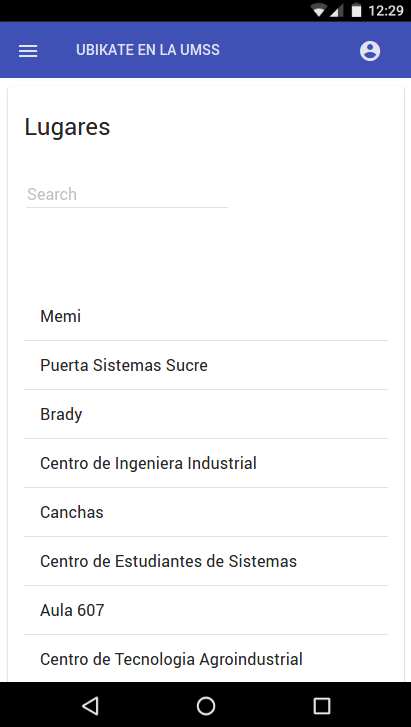
\includegraphics[width=0.3\textwidth]{iteration1/places_index_2}
    \caption{Lista de Lugares}
    \label{fig:places_index}
    \caption*{Fuente: Elaboración propia}
  \end{center}
\end{figure}


\subsubsection{Busqueda de los lugares}
\label{subs:busqueda de los lugares}

Para la implementacion de la busqueda de los lugares, un de los criterios de aceptacion es que sea posible la busqueda usando el nombre del lugar o parte del mismo, es necesario anadir un \emph{URI} adicional a nuestro servicio web, que obtenga de la base de datos un conjunto de lugares que concuerden con el criterio de busqueda, a continuacion se puede ver el URI implementado en la servicio web. \\

\begin{center}
  \begin{lstlisting}[label=endpoint_search_place,caption=Implementacion de la busqueda de lugares en el Servicio Web]

    router.get('places/search/:name', places.getPlacesByName);

  \end{lstlisting}
\end{center}


\subsubsection{Mostrar informacion del lugar}
\label{subs:Mostrar informacion del lugar}

La obtencion de la informacion de un lugar corresponde al URI \emph{places/:id} usando el verbo HTTP \emph{GET}, el cual obtiene la informacion en formato JSON, entonces se necesita mostrar esta informacion en el navegador, para lo cual el template correspondente al URI llegaria a ser \emph{templates/places/show}.

\begin{center}
  \begin{lstlisting}[label=template_places_show,caption=Template para mostrar la informacion de un lugar]
      {{#text.headline}}{{model.name}}{{/text.headline}}
      {{#card.content}}
          {{#paper-list}}
              {{model.description}}
              {{/paper-item}}
                  {{paper-icon "local_phone"}} {{model.phone}}
              {{/paper-item}}
              {{#paper-item class="md-2-line" }}
                  {{paper-icon "layers"}} Piso N# {{model.level}}
              {{/paper-item}}
          {{/paper-list}}
      {{/card.content}}

  \end{lstlisting}
\end{center}

El resultado del template renderizado en el navegador se puede apreciar en la figura \ref{fig:place_show}.

\begin{figure}[H]
  \begin{center}
    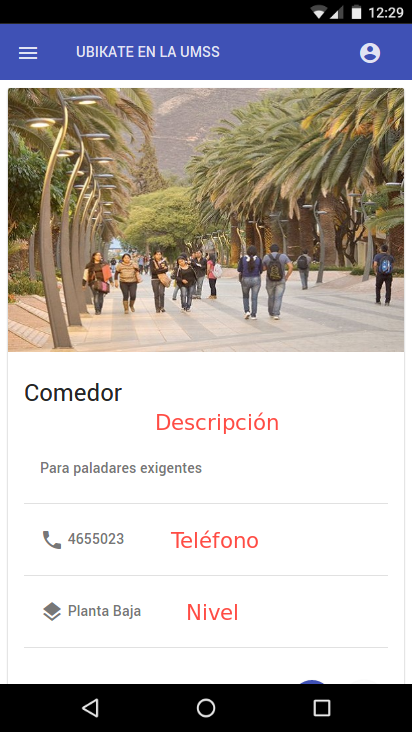
\includegraphics[width=0.3\textwidth]{iteration1/place_show}
    \caption{Vista de la Información de un Lugar.}
    \label{fig:place_show}
    \caption*{Fuente: Elaboración propia}
  \end{center}
\end{figure}




% En la figura \ref{fig:places_index}, se puede observar un
